% "{'classe':('PSI'),'chapitre':'stat_mam','type':('application'),'titre':'Modélisation des actions mécaniques', 'source':'Concours Centrale - MP 2019','comp':('B2-14','C1-05','C2-07'),'corrige':True}"
%\setchapterimage{fig_00.jpg}
\chapter*{Application \arabic{cptApplication} \\ 
Modélisation des actions mécaniques -- \ifprof Corrigé \else Sujet \fi}
\addcontentsline{toc}{section}{Application \arabic{cptApplication} : Modélisation des actions mécaniques  -- \ifprof Corrigé \else Sujet \fi}

\iflivret \stepcounter{cptApplication} \else
\ifprof  \stepcounter{cptApplication} \else \fi
\fi

\setcounter{question}{0}
%\marginnote{Concours Centrale -- MP 2019}
\marginnote[1cm]{
%\UPSTIcompetence[2]{B2-14}
%\UPSTIcompetence[2]{C1-05}
%\UPSTIcompetence[2]{C2-07}
\xpComp{STAT}{02}
}




\section*{Torseur des actions mécaniques transmissibles dans un coussinet}


\ifprof
\else
Un coussinet (ou bague) est un élément technologique permettant de réaliser des liaisons pivot. Suivant les cas d'utilisation d'un système, un chargement sur l'arbre est transmis au coussinet. 

\begin{marginfigure}
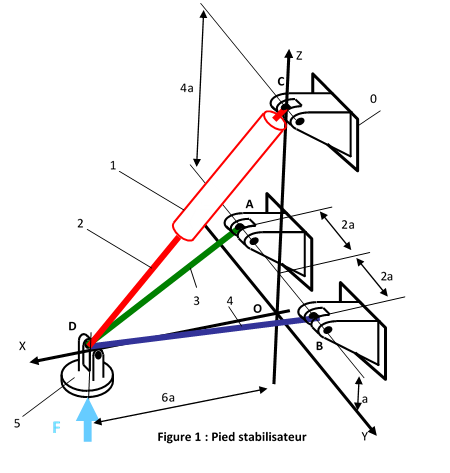
\includegraphics[width=\linewidth]{fig_02}
%\textit{}
\end{marginfigure}
\fi

\begin{center}
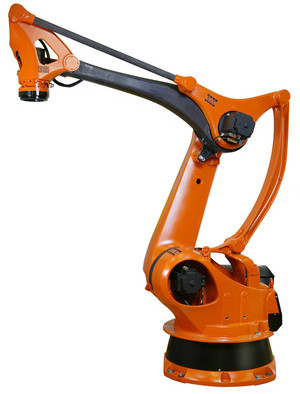
\includegraphics[width=\linewidth]{fig_01}
%\textit{}
\end{center}


On donne le modèle suivant où le champ de pression de l'arbre sur le coussinet est uniforme pour $\theta\in[\pi,2\pi]$ 
On note $R=\dfrac{D}{2}$ le rayon du coussinet. 



\question{Déterminer la résultante des actions mécaniques de 1 sur 3. On la note $\vectf{1}{3}$.}
\ifprof
\begin{corrige}
\begin{enumerate}
\item On commence par exprimer le modèle local d'une action mécanique en $M$ : $\dd \vectf{1}{3} = p(M) \dd S \vect{e_r}$.
\item La pression étant uniforme, on a $p(M)=p$.
\item La géométrie du coussinet étant cylindrique, on se place en coordonnées cylindriques et $\dd S = R\dd \theta \dd z$.  
\item $\theta$ varie sur $[\pi, 2\pi]$ et $z$ sur $[0,L]$. 
\item $\vect{e_r}=\cos\theta\vect{x}+\sin\theta\vect{y}$.
\end{enumerate}
Au final, $\vectf{1}{3}=\int p  \left( \cos\theta\vect{x}+\sin\theta\vect{y}\right)R\dd \theta \dd z$
$=pR\int \left( \cos\theta\vect{x}+\sin\theta\vect{y}\right)\dd \theta \dd z$

$=pR\left( \int  \cos\theta\dd \theta \dd z \vect{x}+\int \sin\theta\dd \theta \dd z   \vect{y}\right)$
$=LpR\left( \int  \cos\theta\dd \theta  \vect{x}+\int \sin\theta\dd \theta   \vect{y}\right)$

$=LpR\left( \left[ \sin \theta \right]^{2\pi}_{\pi}  \vect{x}-\left[\cos \theta \right]^{2\pi}_{\pi}   \vect{y}\right)$

$=LpR\left( -(1-(-1))   \vect{y}\right)$

$=LpR\left( -(1-(-1))   \vect{y}\right)$ $=-2LpR   \vect{y}$ $=-LDp   \vect{y}$.

\end{corrige}
\else
\fi


\question{Déterminer $\vectm{O}{1}{3}\vect{z_N}$.}
\ifprof
\begin{corrige}
\begin{enumerate}
\item On commence par exprimer le modèle local d'une action mécanique en $M$ : $\dd \vectf{1}{3} = p(M) \dd S \vect{e_r}$.
\item Au point $O$, on a $\dd \vectm{O}{1}{3}=\vect{OM}\wedge \dd \vectf{1}{3} =\vect{OM}\wedge \dd \vectf{1}{3} $
\item $\vect{OM}=R\vect{e_r}+z\vect{z}$.
\end{enumerate}
On a alors, $ \vectm{0}{1}{3}\vect{z} =\left( \vect{OM}\wedge \dd \vectf{1}{3}\right) \vect{z}$

$ = \left( \left( R\vect{e_r}+z\vect{z} \right) \wedge  p(M) \dd S \vect{e_r}\right) \vect{z}$

$ = \left(z\vect{z} \wedge  p(M) \dd S \vect{e_r}\right) \vect{z} = 0$


\textbf{Rappel :} le produit mixte est invariant par permutation circulaire : $\left( \vect{a}\wedge \vect{b}\right)\cdot \vect{c} = \left( \vect{c}\wedge \vect{a}\right)\cdot \vect{b} = \left( \vect{b}\wedge \vect{c}\right)\cdot \vect{a}$.
\end{corrige}
\else
\fi

\vspace{.5cm}

On considère maintenant que la pression n'est pas uniforme et vaut au point $M$ $p(M)=p_0\sin\theta$.
\question{Justifier que  $\vectf{1}{3}$ n'a une composante que sur $\vect{y}$.}
\ifprof
\begin{corrige}
Pour des raisons de symétrie du champ de pression, la seule composante sera sur $\vect{y_N}$.
\end{corrige}
\else
\fi


\question{Déterminer la résultante des actions mécaniques de 1 sur 3. On la note $\vectf{1}{3}$. On rappelle que $\sin^2\theta =\dfrac{1-\cos 2\theta }{2}$. }
\ifprof
\begin{corrige}
On cherche donc $\vectf{1}{3} \cdot \vect{y_N}$.
\begin{enumerate}
\item On commence par exprimer le modèle local d'une action mécanique en $M$ : $\dd \vectf{1}{3} = p(M) \dd S \vect{e_r}$.
\item La pression étant uniforme, on a $p(M)=p_0 \sin\theta$.
\item La géométrie du coussinet étant cylindrique, on se place en coordonnées cylindriques et $\dd S = R\dd \theta \dd z$.  
\item $\theta$ varie sur $[\pi, 2\pi]$ et $z$ sur $[0,L]$. 
\end{enumerate}

On a  $\dd \vectf{1}{3} \cdot \vect{y_N} = p(M) \dd S \vect{e_r} \cdot \vect{y_N} =p_0 \dd S  \sin^2 \theta $. 

On a donc $\vectf{1}{3} \cdot \vect{y_N} = \int  p_0  \sin^2 \theta  R\dd \theta \dd z $
$ =   p_0 R L \int \dfrac{1-\cos 2\theta }{2}   \dd \theta$
$ =   \dfrac{1}{2}p_0 R L \left[\theta-\dfrac{1}{2}\sin 2\theta \right]^{2\pi}_{\pi} $
$ =   \dfrac{1}{2}p_0 R L {\pi} $
$ =   \dfrac{1}{4}p_0 D L {\pi} $.
\end{corrige}
\else
\fi



\ifcolle
\else
\ifprof
\else
\marginnote{
\begin{solution}
\begin{enumerate}
 \item $\vectf{1}{3}=-LDp   \vect{y}$.
 \item $\vectm{O}{1}{3}\vect{z_N}=0$.
 \item 
 \item $\vectf{1}{3} \cdot \vect{y_N} =-\dfrac{p_0 D L {\pi} }{4}$.
\end{enumerate}
\end{solution}}
\fi
\fi

\newpage

\section*{Détermination des efforts dans une structure étayée}
\marginnote{
\xpComp{STAT}{01}
\xpComp{STAT}{03}
\xpComp{STAT}{04}
}
\ifprof
\else

\begin{marginfigure}
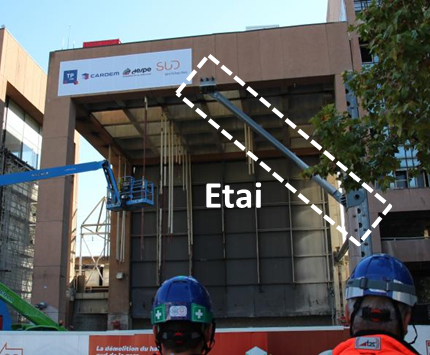
\includegraphics[width=\linewidth]{fig_03b}
%\textit{}
\end{marginfigure}

Lors de la démolition d'une partie de la gare de Lyon Part-Dieu (en 2018), des étais ont du être posés afin de soutenir la structure supérieure. 


Dans le but de dimensionner les étais, il est nécessaire de déterminer les actions mécanique dans chacune des liaisons. 


\begin{marginfigure}
\centering
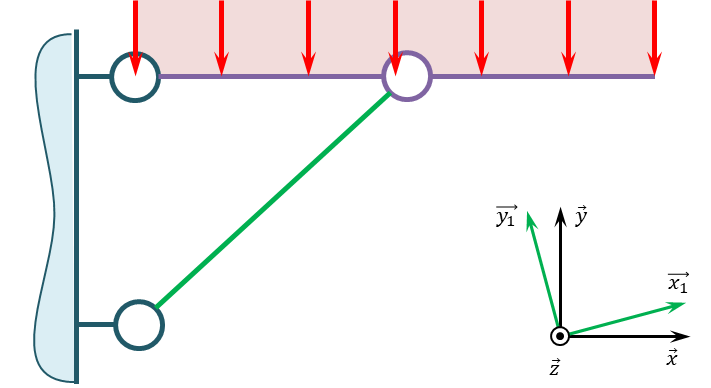
\includegraphics[width=\linewidth]{fig_04a}
\caption{Modélisation initiale}
\end{marginfigure}


\begin{marginfigure}
\centering
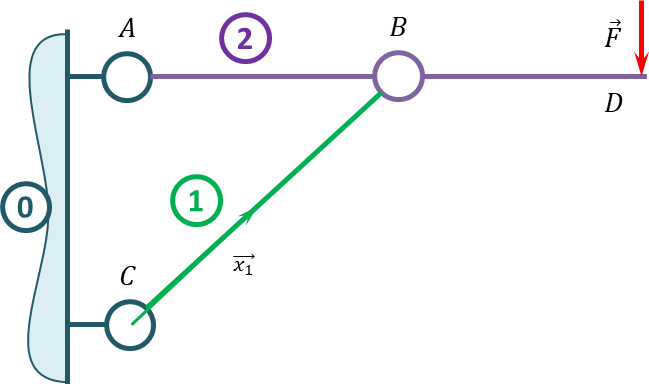
\includegraphics[width=\linewidth]{fig_04b}
\caption{Modélisation retenue}
\end{marginfigure}

Pour cela, on utilise la modélisation ci-contre. 



On a $\vect{AB}=a \vect{x}$,  $\vect{BD}=b \vect{x}$ et  $\vect{CB}=L \vect{x_1}$.
\fi

\question{Tracer le graphe d'analyse du système (graphe des liaisons et actions extérieures).}
\ifprof
\begin{corrige}
\begin{center}
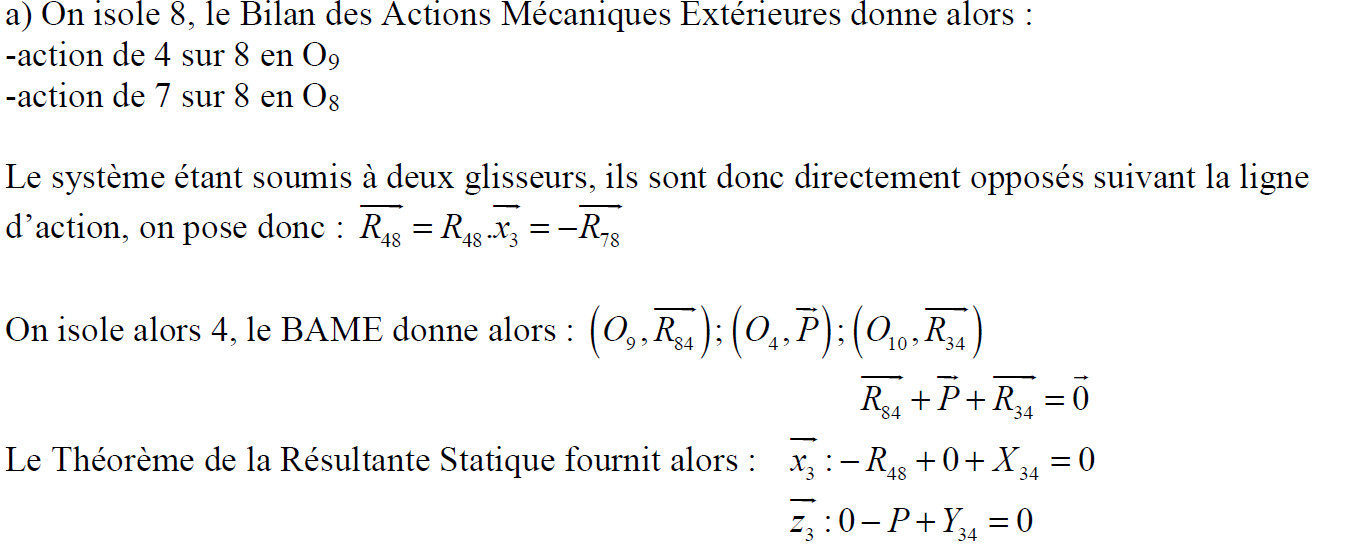
\includegraphics[width=\linewidth]{cor_01}
%\textit{}
\end{center}

\end{corrige}
\else
\fi

\question{Proposer une stratégie permettant de déterminer les actions mécaniques dans les liaisons.}
\ifprof
\begin{corrige}
Ici, il s'agit de déterminer les actions mécaniques dans toutes les liaisons. Il faudra donc isoler successivement toutes les pièces et réaliser un PFS pour chacune d'entre elles. Cependant, il y a quand même une stratégie d'isolement à avoir : \textbf{il faut commencer par isoler les solides soumis à deux glisseurs}. En effet, d'après le PFS, lorsqu'un solide est soumis à deux glisseurs, les deux forces sont de même norme, de même direction (droite passant par le point d'application des deux glisseurs) et de sens opposé. 

La stratégie est donc la suivante : 
\begin{itemize}
\item on isole 1 et on réalise le PFS. 
\item on isole 2 et on réalise le PFS en B. 
\end{itemize} 


\end{corrige}
\else
\fi


\question{Déterminer les actions mécaniques dans les liaisons en fonction de $F$.}
\ifprof
\begin{corrige}

\textbf{On isole 1}.
\textbf{On réalise le BAME :}
\begin{itemize}
\item $\torseurstat{T}{0}{1}$;
\item $\torseurstat{T}{2}{1}$.
\end{itemize}
\textbf{D'après le PFS pour un solide soumis à 2 glisseurs, on a : }
$\torseurstat{T}{0}{1} + \torseurstat{T}{2}{1} = {0}$. 

\textbf{Résolution :} 
$ \torseurstat{T}{0}{1} = -\torseurstat{T}{2}{1}  = \torseurl{F_{01}\vect{x_1}}{\vect{0}}{A}$.

\end{corrige}

\begin{corrige}

\textbf{On isole 2}.
\textbf{On réalise le BAME :}
\begin{itemize}
\item $\torseurstat{T}{0}{2} =\torseurl{X_{02}\vect{x} +Y_{02}\vect{y}  }{\vect{0}}{A} $ $=\torseurl{X_{02}\vect{x} +Y_{02}\vect{y}  }{-aY_{02}\vect{z}}{A} $;
\item $\torseurstat{T}{1}{2} = \torseurl{F_{01}\vect{x_1}  }{\vect{0}}{B} $;
\item $\torseurstat{T}{\text{ext}}{2} = \torseurl{-F\vect{y}  }{\vect{0}}{C} $ $= \torseurl{-F\vect{y}  }{-Fb\vect{z}}{C}$.
\end{itemize}
\textbf{D'après le PFS pour un solide soumis à 2 glisseurs, on a : }

$\torseurstat{T}{0}{2} + \torseurstat{T}{1}{2}+\torseurstat{T}{\text{ext}}{2} = {0}$.

 \textbf{Résolution :}

$\left\{ \begin{array}{l}
X_{02}+F_{01}\cos\alpha  = 0 \\
Y_{02}+F_{01}\sin\alpha  -F= 0 \\
-aY_{02}-Fb  = 0 \\
\end{array}
\right.$


$
\Leftrightarrow 
\left\{ \begin{array}{l}
X_{02}=-F_{01}\cos\alpha  =-F\dfrac{a+b}{a\tan\alpha} \\
F_{01}  =\dfrac{F-Y_{02}}{\sin\alpha}=F\dfrac{a+b}{a\sin\alpha} \\
Y_{02} = -\dfrac{b}{a}F  \\
\end{array}
\right.$

\end{corrige}

\else
\fi


%\noindent\footnotesize
%\fbox{\parbox{.9\linewidth}{
%Éléments de corrigé : 
%\begin{enumerate}\setcounter{enumi}{2}
%    \item $X_{02}=-F\dfrac{a+b}{a\tan\alpha}$, $F_{01}  =F\dfrac{a+b}{a\sin\alpha}$, $Y_{02} = -\dfrac{b}{a}F$.
%\end{enumerate}}}
%\normalsize


\ifcolle
\else
\ifprof
\else
\marginnote{
\begin{solution}
\begin{enumerate}[wide, labelwidth=!, labelindent=0pt]
\setcounter{enumi}{2}
\item $X_{02}=-F\dfrac{a+b}{a\tan\alpha}$, $F_{01}  =F\dfrac{a+b}{a\sin\alpha}$, $Y_{02} = -\dfrac{b}{a}F$.
\end{enumerate}
\end{solution}}
\fi
\fi

\ifprof
\else
\begin{marginfigure}
\centering

\includegraphics[width=3cm]{Cy_11_Ch_01_01_qr}
\end{marginfigure}
\fi


